\subsection{Use case diagram}
	A global picture of the system interaction with actors is provided here by means of use case diagrams. Following, an analysis of the most interesting use case situations derived from scenarios is presented.

	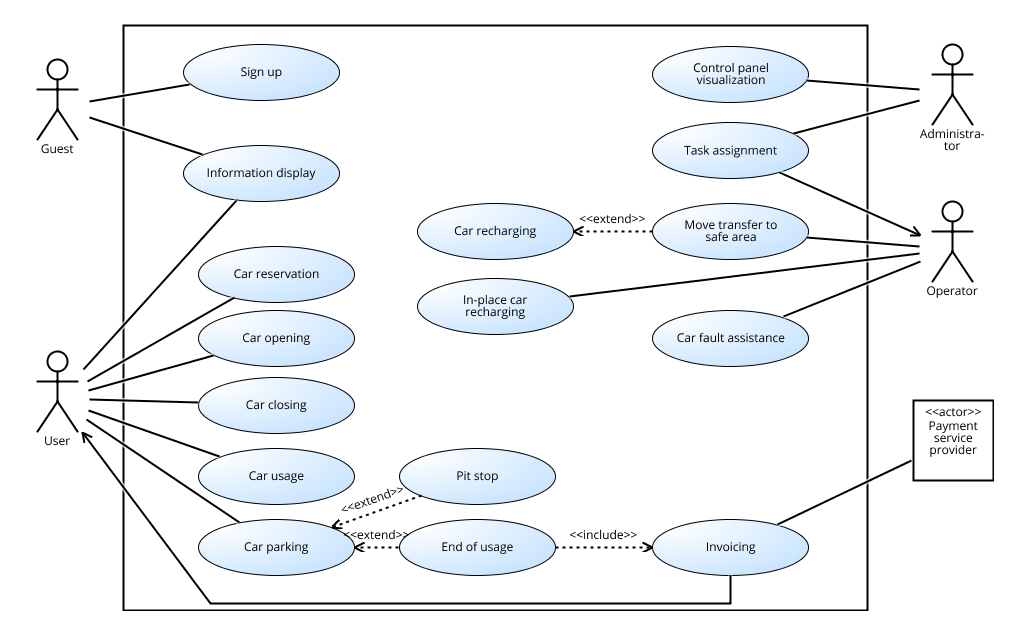
\includegraphics[width=\textwidth]{img/use_case.png}

	\subsubsection{Use case 1: Reserve a car}
		\begin{description}
			\item[Name] Reserve a car
			\item[Actors] \hfill
				\begin{description}
					\item[User] The user who wants to reserve a car.
				\end{description}
			\item[Entry condition] The user decides to reserve a car to take in the next hour.
			\item[Flow of events] \hfill
				\begin{enumerate}
					\item The user logs in into the mobile app and goes to the reservation section. \item The system automatically retrieves and displays the location of the user, but they can specify a different location if needed.
					\item The system displays the position of the available cars close to the selected location.
					\item The user selects a car and confirm the reservation.
				\end{enumerate}
			\item[Exit condition] The system reserves the car for the user.
			\item[Exceptions] \hfill
				\begin{itemize}
					\item \textbf{The system is not able to locate the user automatically.} The user is required to insert a position manually.
					\item \textbf{The system is not able to find a position inserted manually.} The user is informed and the operation is aborted.
					\item \textbf{There are no available cars.} The user is informed and the operation is aborted.
					\item \textbf{The user cancels the operation before confirming.} The reservation process is not completed and the car remains available to other users.
				\end{itemize}
			\item[Special Requirements] None.
		\end{description}

	\subsubsection{Use case 2: Park in known safe area}
		\begin{description}
			\item[Name] Park in known safe area
			\item[Actors] \hfill
				\begin{description}
					\item[User] The user of the car.
					\item[Car] The car in use.
				\end{description}
			\item[Entry condition] The user is driving and has reached their destination. They know a safe area close to the destination.
			\item[Flow of events] \hfill
				\begin{enumerate}
					\item The safe area is free and the user parks in it.
					\item As the car is turned off, the system detects it is in a safe area.
					\item The system asks the user if he wants to keep the car or to end the ride.
					\item The user selects to end the ride.
					\item The user exits the car.
					\item The system closes the car.
					\item The system charges the user for the ride.
				\end{enumerate}
			\item[Exit condition] The user leaves the car and the car becomes available to other users.
			\item[Exceptions] \hfill
				\begin{itemize}
					\item \textbf{The safe area is taken.} The user can't end their ride and this operation is aborted.
					\item \textbf{The car is badly parked.} ??? % TODO
					\item \textbf{The user selects to keep the car when prompted.} The user keeps being charged and the car is not made available for other users.
				\end{itemize}
			\item[Special Requirements] None. % TODO are there any?
		\end{description}

	\subsubsection{Use case 3: Park with money saving option}
		\begin{description}
			\item[Name] Park with money saving option
			\item[Actors] \hfill
			\begin{description}
				\item[User] The user of the car.
				\item[Car] The car in use.
			\end{description}
			\item[Entry condition] The user selects the \textit{money saving option} at some point of their ride and insert their destination.
			\item[Flow of events] \hfill
			\begin{enumerate}
				\item The system indicates the user the suggested safe area for their destination.
				\item The user parks in the suggested safe area.
				% from here, same as Use case 2:
				\item As the car is turned off, the system detects it is in a safe area.
				\item The system asks the user if he wants to keep the car or to end the ride.
				\item The user selects to end the ride.
				\item The user exits the car.
				\item The system closes the car.
				\item The system charges the user for the ride. A discount is applied for using the \textit{money saving option}.
			\end{enumerate}
			\item[Exit condition] The user leaves the car and the car becomes available to other users.
			\item[Exceptions] \hfill
			\begin{itemize}
				\item \textbf{The suggested safe area becomes taken while the user is driving.} The system selects another safe area and notifies the user of the new suggestion.
				\item \textbf{The user parks in another safe area.} The system notifies the user that they will not receive a discount. If the user decides to end the ride anyway, the system charges them without applying the \textit{money saving option} discount.
				\item \textbf{The destination of the user changes.} The user selects a new destination and the system indicates another suggestion.
				\item \textbf{The user disables the \textit{money saving option} while driving.} The suggested safe area stops being displayed and the ride continues as normal.
			\end{itemize}
			\item[Special Requirements] The \textit{money saving option} must be selected before stopping the car in a parking area. % FIXME necessary?
		\end{description}

	\subsubsection{Use case 4: Park in a recharging area}
		\begin{description}
			\item[Name] Park in a recharging area
			\item[Actors] \hfill
			\begin{description}
				\item[User] The user of the car.
				\item[Car] The car in use.
			\end{description}
			\item[Entry condition] The user is about to park in a recharging area.
			\item[Flow of events] \hfill
			\begin{enumerate}
				\item The user parks the car in the recharging area.
				% same as parking in safe area
				\item As the car is turned off, the system detects it is in a safe area.
				\item The system asks the user if he wants to keep the car or to end the ride.
				\item The user selects to end the ride.
				\item The user exits the car.
				\item The system closes the car.
				\item The system charges the user for the ride.
				% /same as parking in safe area
				\item The user plugs the car into the power grid through the supply point installed in the parking space.
				\item The system detects the car is recharging.
				\item The system modifies the charge applied to the user for the ride. A 30\% discount is applied to promote virtuous behaviors.
			\end{enumerate}
			\item[Exit condition] The user leaves the car and the car becomes available to other users.
			\item[Exceptions] \hfill
			\begin{itemize}
				\item \textbf{The user does not plug the car into the power grid.} The user is charged as if they parked in a safe area.
			\end{itemize}
			\item[Special Requirements] The user plugs in the car within 5 minutes from the moment they exits the car. Otherwise the discount is not applied.
		\end{description}
